\documentclass[12pt,letter]{article}
\usepackage{mathptmx} % added for time new roman font
\usepackage[left=1in,right=1in,top=1in,bottom=1in]{geometry}
\usepackage[latin1]{inputenc}
\usepackage{amsmath}
\usepackage[final]{pdfpages}

\usepackage[textsize=tiny]{todonotes}

% defines all example enviorment
\usepackage[framemethod=tikz]{mdframed} % added for the box around examples
\newtheorem{ex}{Example}
\numberwithin{ex}{section} % allows for the use of example numbers that lign up with the section numbers
\newenvironment{example}{\begin{mdframed}[middlelinewidth=0.5mm]\begin{ex}\normalfont}{\end{ex}\end{mdframed}}

% defines all review enviorment
\usepackage[framemethod=tikz]{mdframed} % added for the box around examples
\newtheorem{re}{Review}
\numberwithin{re}{section} % allows for the use of example numbers that lign up with the section numbers
\newenvironment{review}{\begin{mdframed}[middlelinewidth=2mm,roundcorner=20pt]\begin{re}\normalfont}{\end{re}\end{mdframed}}

% defines the quotation enviorment 
\usepackage{xcolor}
\newcommand{\quotebox}[2]{\begin{center}\fcolorbox{white}{blue!15!gray!15}{\begin{minipage}{0.9\linewidth}\vspace{10pt}\center\begin{minipage}{0.8\linewidth}{\space\Huge``}{#1}{\Huge''}{\break\null\hfill} {\small #2}  \end{minipage}\medbreak\end{minipage}}\end{center}}

% defines the definition enviorment 
\newcommand{\definitionbox}[2]{\begin{center}\fcolorbox{white}{blue!15!gray!15}{\begin{minipage}{0.9\linewidth}\vspace{10pt}\center\begin{minipage}{0.8\linewidth} {{\textbf{Definition} - }{#1}: {#2}}\end{minipage}\medbreak\end{minipage}}\end{center}}

\usepackage{amsfonts}
\usepackage{amssymb}
\usepackage{graphicx}
\usepackage{float}
\usepackage{booktabs}
%\usepackage{parskip} % remove all the paragraph indents
\usepackage{xfrac}
\usepackage{upgreek}
\usepackage{wrapfig}
\usepackage{setspace}
\usepackage[colorlinks=true]{hyperref}
\usepackage{textcomp} 
\usepackage{multicol} 
\usepackage{enumitem}		% added for spacing in itemize lists
\usepackage[numbered,framed]{matlab-prettifier}		% added for matlab code
\let\ph\mlplaceholder % shorter macro
\lstMakeShortInline"
\lstset{
  style              = Matlab-editor,
  basicstyle         = \mlttfamily,
  escapechar         = ",
  mlshowsectionrules = true,
}

\usepackage{color} % color added for editing
\newcommand{\bl}[1]{\textcolor[rgb]{0.00,0.00,1.00}{#1}}
\newcommand{\gr}[1]{\textcolor[rgb]{0.00,0.50,0.00}{#1}}
\newcommand{\rd}[1]{\textcolor[rgb]{0.75,0.00,0.00}{#1}}

\usepackage{fancyhdr}
\pagestyle{fancy}
\fancyfoot{} % clear all footer fields
\fancyfoot[LE,RO]{Page \thepage} 
\fancyfoot[RE,LO]{}

%%%%%%%		define the symbols for positive directions		%%%%%%
\makeatletter													%%	
																%%					
\newcommand*\curveplus{% positive counterclockwise				%%
  \mathbin{\rotatebox[origin=c]{90}{$\m@th\curvearrowleft$}+}}	%%
																%%
\newcommand*\rightplus{% positive right							%%
  \mathpalette\@rightplus\relax}								%%
\newcommand*\@rightplus[1]{%									%%
  \mathbin{\vcenter{\hbox{$\m@th\overset{#1+}{\to}$}}}}			%%
																%%	
\newcommand*\upplus{% positive up								%%
  \mathbin{+\mathord\uparrow}}									%%
																%%			
\newcommand*\downplus{% positive down							%%		
  \mathbin{+\mathord\downarrow}}								%%
  																%%		
\newcommand*\downrightplus{% positive down and right			%%	
  \mathbin{+ \rotatebox[origin=c]{-30}{$\m@th\rightarrow$}}}	%%
\makeatother 													%%	
%%%%%%%%%%%%%%%%%%%%%%%%%%%%%%%%%%%%%%%%%%%%%%%%%%%%%%%%%%%%%%%%%%


\usepackage{mathtools}          %loads amsmath as well added for the piece wise function
\DeclarePairedDelimiter\Floor\lfloor\rfloor
\DeclarePairedDelimiter\Ceil\lceil\rceil

 
\newcounter{NumberInTable}
\newcommand{\LTNUM}{\stepcounter{NumberInTable}{(\theNumberInTable)}}

\newcommand{\Laplace}[1]{\ensuremath{\mathcal{L}{\left[#1\right]}}}
\newcommand{\InvLap}[1]{\ensuremath{\mathcal{L}^{-1}{\left[#1\right]}}}
\renewcommand{\textuparrow}{$\uparrow$}

\numberwithin{equation}{section}	% added so the equsation numbers are section.# and start at section.1

\begin{document}
%	
%	\large{}
%	
%	\title{\vspace{-2cm} Chapter 1: Basic concepts of Control Theory}
%	\date{}
%	\maketitle

	% set the section number, along with figure and equation numbers
	\setcounter{section}{4}	
	\setcounter{figure}{0}   
	\renewcommand\thefigure{\thesection.\arabic{figure}}


\section{Performance Indicators}

Performance indicators are used to judge the quality of a control system. 

\subsection{1\textsuperscript{st}-order System Generic Performance Indicators}


Generic performance indicators are:
\begin{itemize}
	\item steady-state value $x_{ss} = \lim\limits_{t \rightarrow \infty} x(t)$
	\item steady-state error $e_{ss} = \lim\limits_{t \rightarrow \infty} e(t)$ where  $e(t) = f(t) - x(t)$
\end{itemize}
To expand on the error definition, $e(t) = f(t) - x(t)$, consider a step response where $x(\infty) =1$ and $f(\infty) =1$, therefore $e(\infty)=0$. 

For a 1\textsuperscript{st}-order system, $x_{ss}$ and $e_{ss}$ can be found using the final value theorem and exist in both the time domain and the s-domain. Recall the final value theorem for  $x_{ss}$ and $e_{ss}$ leads to
\begin{equation}
x_{ss} = \lim\limits_{s \rightarrow 0} s X(s)
\end{equation}
\begin{equation}
e_{ss} = \lim\limits_{s \rightarrow 0} s E(s)
\end{equation}
Therefore, starting at the transfer function of a 1\textsuperscript{st}-order system
\begin{equation}
G(s) = \frac{1}{Ts+1}
\end{equation}
we can expand on this to show
\begin{align}
X(s) &= G(s)F(s) \\
&= \frac{1}{Ts +1}F(s) \nonumber
\end{align}
next, the error is s-domain is shown to be
\begin{align}
E(s) &= F(s) - X(s) \\
&= F(s) - G(s)F(s) \\ \nonumber
&= \big( 1-G(s) \big) F(s) \\ \nonumber
&= \frac{Ts}{Ts +1} F(s) \nonumber
\end{align}
Again, these are general terms for a 1\textsuperscript{st}-order system. 


\subsubsection{Step response 1\textsuperscript{st}-order system performance indicators}

\begin{figure}[H]
	\centering
	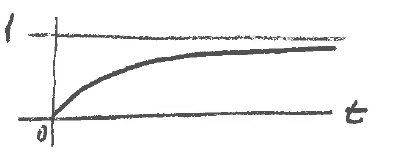
\includegraphics[width=2.5in]{../figures/step_response_with_steady_state_error}
\end{figure}



For a 1\textsuperscript{st}-order system subjected to a step response, we want to find $x_{ss}$ and $e_{ss}$ and we know the transfer function is defined as  
\begin{equation}
G(s) = \frac{1}{T s + 1}
\end{equation}
while the equation of motion is
\begin{equation}
T \dot{x} + x = F(s)
\end{equation}
Where the step function is defined as
\begin{equation}
f(t) =1, \; t > 0
\end{equation}
therefore, the system response is
\begin{equation}
x(t) =1-e^{-t/T} 
\end{equation}
while the steady-state response is
\begin{align}
x_{ss} &= \lim\limits_{t \rightarrow \infty} \\
&= 1 \nonumber
\end{align}
Next, the error as a function of time is 
\begin{align}
e(t) &= 1-(1-e^{-t/T}) \\
&= e^{-t/T} \nonumber
\end{align}
while the steady-state error is
\begin{align}
e_{ss} &= \lim\limits_{t \rightarrow \infty}e(t) \\
&= \lim\limits_{t \rightarrow \infty}e^{t/T}  \nonumber \\
&= 0 \nonumber
\end{align}

These same solutions can be found in the s-domain where the step function is $F(s)=\frac{1}{s}$. Consider the s-domain expression solved for $X(s)$, 
\begin{equation}
X(s) = \frac{1}{Tx +1} \cdot \frac{1}{s} 
\end{equation}
the steady-state error is shown to be
\begin{align}
x_{ss} &= \lim\limits_{s \rightarrow 0} s \frac{1}{Ts+1} \cdot \frac{1}{s} \\
&= \lim\limits_{s \rightarrow 0} \frac{1}{Ts+1}   \nonumber \\
&= 1    \nonumber 
\end{align}
Next, we can build the s-domain representation of the error as
\begin{align}
E(s) &= \frac{Ts}{Ts +1} \cdot \frac{1}{s} \\
&= \frac{T}{Ts +1}  \nonumber 
\end{align}
solving for the steady-state error results in
\begin{align}
e_{ss} &= \lim\limits_{s \rightarrow 0}  s \frac{T}{Ts+1} \\
&= 0   \nonumber 
\end{align}

\subsubsection{Impulse response 1\textsuperscript{st}-order system performance indicators}

\begin{figure}[H]
	\centering
	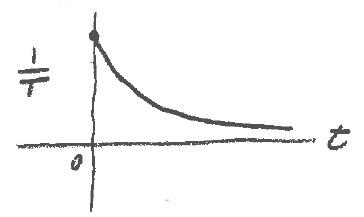
\includegraphics[width=2.5in]{../figures/impulse_response_with_steady_state_error}
\end{figure}



For a 1\textsuperscript{st}-order system subjected to a impulse response, we want to find $x_{ss}$ and $e_{ss}$. The impulse function is defined as
\begin{equation}
f(t) = \delta(t)
\end{equation}
therefore, the response is
\begin{equation}
x(t) =\frac{1}{T} e^{-t/T}
\end{equation}
where the steady-state response is
\begin{equation}
x_{ss} = 0
\end{equation}
The error is
\begin{equation}
e(t) = \delta(t) - \frac{1}{T} e^{-t/T}
\end{equation}
Lastly, the steady-state error is
\begin{align}
e_{ss} &= \lim\limits_{t \rightarrow \infty}e(t) \\
&= 0 \nonumber
\end{align}

These same solutions can be found in the s-domain where the impulse function is $F(s)=1$. Consider the s-domain expression solved for $X(s)$, 
\begin{equation}
X(s) = \frac{1}{Ts +1} 
\end{equation}
the steady-state error is shown to be
\begin{align}
x_{ss} &= \lim\limits_{s \rightarrow 0} s \frac{1}{Ts+1}  \\
&= 0    \nonumber 
\end{align}
The s-domain error is expressed as
\begin{equation}
E(s) = \frac{T}{Ts +1} 
\end{equation}
which leads to the steady-state error value
\begin{align}
e_{ss} &= \lim\limits_{s \rightarrow 0}  s \frac{T}{Ts+1} \\
&= 0   \nonumber 
\end{align}







\subsubsection{Ramp response 1\textsuperscript{st}-order system performance indicators}

\begin{figure}[H]
	\centering
	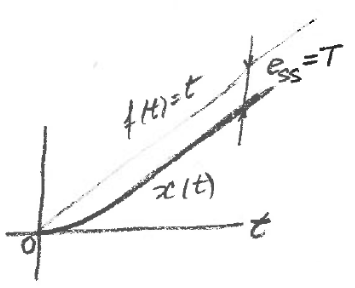
\includegraphics[width=2.5in]{../figures/ramp_response_with_steady_state_error}
\end{figure}



For a 1\textsuperscript{st}-order system subjected to a ramp response, we want to find $x_{ss}$ and $e_{ss}$. The impulse function is defined as
\begin{equation}
f(t) = t
\end{equation}
therefore, the response is
\begin{equation}
x(t) = t - T(1-e^{-t/T})
\end{equation}
which leads to the steady-state response
\begin{equation}
x_{ss} =  \infty 
\end{equation}
which means that there is no steady-state value. The error is
\begin{equation}
e(t) = T(1-e^{-t/T})
\end{equation}
Lastly, the steady-state error is
\begin{align}
e_{ss} &= \lim\limits_{t \rightarrow \infty}e(t)  \\
&= T - \lim\limits_{t \rightarrow \infty}e^{-t/T} \nonumber \\
&= T \nonumber
\end{align}
as $\lim\limits_{t \rightarrow \infty}e^{-t/T} = 0$.

These same solutions can be found in the s-domain where the ramp function is $F(s)=\frac{1}{s^2}$. Consider the s-domain expression solved for $X(s)$, 
\begin{equation}
X(s) = \frac{1}{Ts +1} \cdot \frac{1}{s^2} 
\end{equation}
the steady-state error is shown to be
\begin{align}
x_{ss} &= \lim\limits_{s \rightarrow 0} s \frac{1}{Ts+1} \cdot \frac{1}{s^2} \\
&= \lim\limits_{s \rightarrow 0} \frac{1}{Ts+1} \cdot \frac{1}{s}  \nonumber \\
&= \infty    \nonumber 
\end{align}
therefore, there is no steady-state value. The s-domain error is expressed as
\begin{align}
E(s) &= \frac{Ts}{Ts +1} \cdot \frac{1}{s^2} \\
&= \frac{T}{Ts +1} \cdot \frac{1}{s}  \nonumber 
\end{align}
which leads to the steady-state error value
\begin{align}
e_{ss} &= \lim\limits_{s \rightarrow 0}  s \frac{T}{Ts+1} \cdot \frac{1}{s} \\
&= \lim\limits_{s \rightarrow 0}   \frac{T}{Ts+1} \nonumber \\
&= T   \nonumber 
\end{align}


\subsection{1\textsuperscript{st}-order System Specific Performance Indicators}


Specific performance indicators exist. They depend on system order and excitation type. Examples are:
\begin{itemize}
	\item rise-time $ \rightarrow t_r$
	\item delay time  $ \rightarrow t_d$
	\item settling time $ \rightarrow t_s$
	\item decay time / half-time $ \rightarrow t_{1/2}$
\end{itemize}

For a step response, consider the system displacement
\begin{equation}
x(t) = 1-e^{-t/T}
\end{equation}
that is plotted as
\begin{figure}[H]
	\centering
	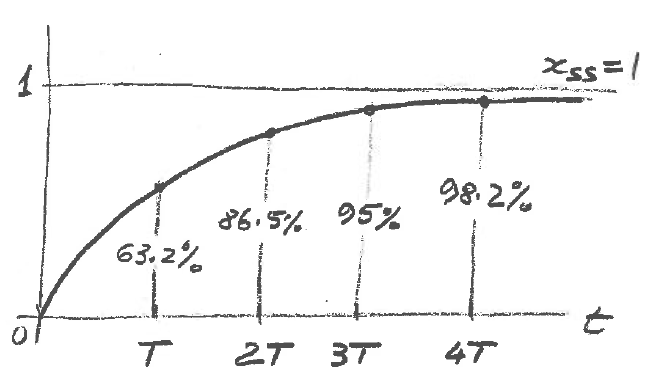
\includegraphics[width=4.5in]{../figures/system_specific_performance_indicator_rise_time}
\end{figure}

The rise-time ($t_r$) of a system
\begin{itemize}
\item to rise 63.2\% of $x_ss$ is $t_{r\_63.2\%} = T$
\item to rise 86.5\% of $x_ss$ is $t_{r\_86.5\%} = 2T$
\item to rise 95\% of $x_ss$ is $t_{r\_95\%} = 3T$
\item to rise 98.2\% of $x_ss$ is $t_{r\_98.2\%} = 4T$
\end{itemize}
in general, $1-e^{-t/T} = x \rightarrow t = -T \ln(1-x)$ 

The delay time ($t_d$) is the time it takes to rise to 50\% of $x_{ss}$, 

\begin{align}
x(t) &= 1-e^{-t/T} \\
&= 0.5 \nonumber
\end{align}
therefore, solving for $t=t_d$,
\begin{align}
e^{-t_d/T} &= 0.5 \\
\frac{-t_d}{T} &= \ln(0.5) \nonumber \\
t_d &= -T \ln(0.5) \nonumber \\
t_d &= 0.693 T \nonumber \\
t_d & \approx 0.7T \nonumber 
\end{align}

The settling time ($t_s$) is the time its takes $x$ to get within $\epsilon \%$ of $x_{ss}$.
\begin{figure}[H]
	\centering
	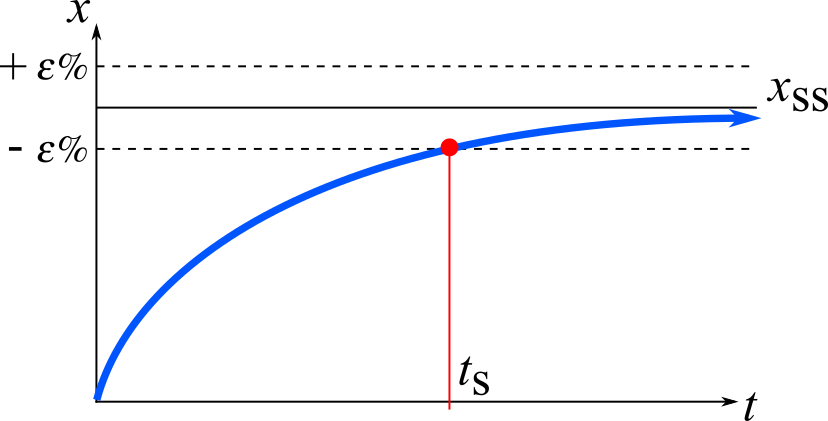
\includegraphics[]{../figures/performance_indicator_settling_time}
\end{figure}

A more precise estimator is the rise time to any selected $x$ which can be defined as
\begin{align}
x_{ss}(1-e^{-t/T})&=x \\
 e^{(-t/T)} &= 1-\frac{x}{x_{ss}} \nonumber \\ 
-t/T &= \log \bigg[ 1-\frac{x}{x_{ss}} \bigg]  \nonumber \\ 
t &= -T \log \bigg[ 1-\frac{x}{x_{ss}} \bigg] \nonumber 
\end{align}

\subsubsection{Impulse Response Specific Performance Indicators}

\begin{figure}[H]
	\centering
	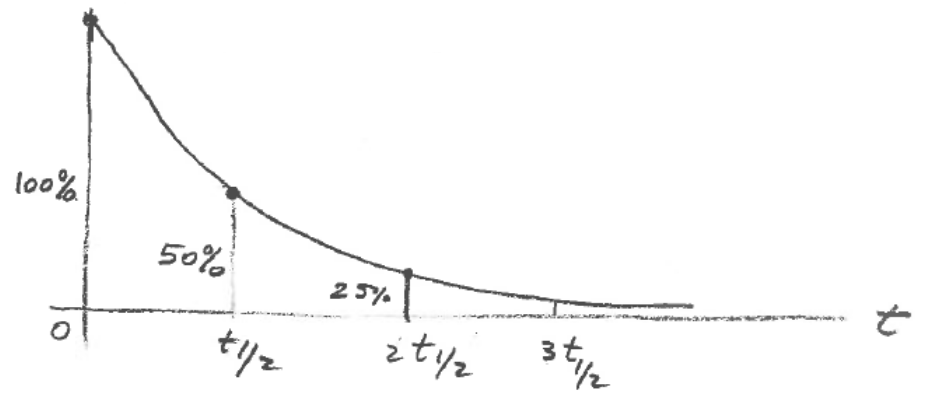
\includegraphics[width=4.5in]{../figures/system_specific_performance_indicator_decay_time}
\end{figure}

The half-cycle decay time ($t_{1/2}$) is an impulse response specific performance indicator. Given that the system response to an impulse is
\begin{equation}
x(t) = \frac{1}{T} e^{-t/T}
\end{equation}
the half-life decay time is where $e^{-t/T} = \frac{1}{2}$, therefore
\begin{align}
t_{1/2} &= - \ln \bigg(\frac{1}{2} \bigg) T \\
&\approxeq 0.693T \nonumber
\end{align}
Note that the signal continues to decay by half of its value after each additional $t_{1/2}$.





\begin{example}

\textbf{SIMULINK Tutorial on Measuring Performance Indicators}

Build the simple 1\textsuperscript{st}-order system as shown below
\begin{figure}[H]
	\centering
	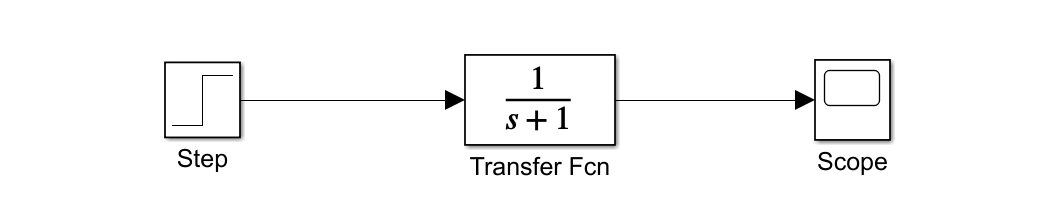
\includegraphics[width=4.5in]{../figures/Simulink_step_model_transfer}
\end{figure}
Open the scope and press the `Cursor Measurements' button to activate the cursors.

\begin{figure}[H]
	\centering
	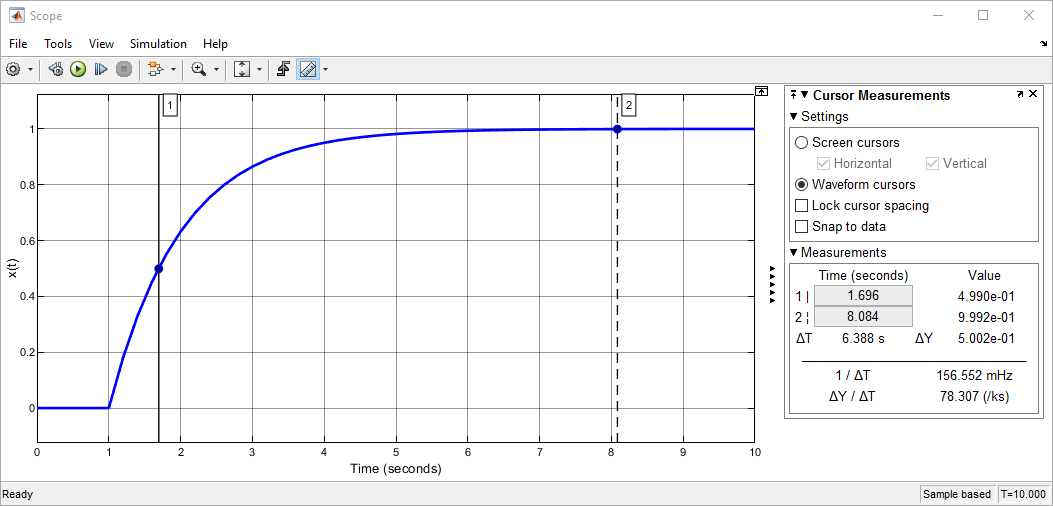
\includegraphics[width=6.0in]{../figures/Simulink_step_model_transfer_cursor_measurements}
\end{figure}




To measure the delay time $t_d$, place the first cursor around the point where `Value' measurement is closest to 0.5. $x(t) = 0.5$. Read the `Time' value. This is estimate for $t_d$ . It gives the value $t_d = 0.70$ sec, as the step function happens at 1 sec. 

The second cursor can be used to get the settling time $t_s$ . We are going to use the 1\% definition of $t_d$ . This means that the response should be around 0.99, or 9.9e-1. Reading the corresponding time value, we get $t_s \approx$  7.0 sec. 

\end{example}


\subsection{2\textsuperscript{nd}-order System Generic Performance Indicators}

%Generic performance indicators are:
%\begin{itemize}
%	\item steady-state value $x_{ss} = \lim\limits_{t \rightarrow \infty} x(t)$
%	\item steady-state error $e_{ss} = \lim\limits_{t \rightarrow \infty} e(t)$ where  $e(t) = f(t) - x(t)$
%\end{itemize}
%To expand on the error definition, $e(t) = f(t) - x(t)$, consider a step response where $x(\infty) =1$ and $f(\infty) =1$, therefore $e(\infty)=0$. 
%
%For a 1\textsuperscript{st}-order system, $x_{ss}$ and $e_{ss}$ can be found using the final value theorem and exist in both the time domain and the s-domain. Recall the final value theorem for for  $x_{ss}$ and $e_{ss}$ leads to
%\begin{equation}
%x_{ss} = \lim\limits_{s \rightarrow 0} s X(s)
%\end{equation}
%\begin{equation}
%e_{ss} = \lim\limits_{s \rightarrow 0} s E(s)
%\end{equation}



Again, starting at the equation of motion
\begin{equation}
\ddot{x} + 2 \zeta \omega_n \dot{x} + \omega_n^2 x = \omega_n^2 f(t)
\end{equation}
and transfer function of a 2\textsuperscript{nd}-order system
\begin{equation}
G(s) = \frac{\omega_n^2}{s^2 + 2 \zeta \omega_n s + \omega_n^2}
\end{equation}
we can expand on this to show
\begin{align}
X(s) &= G(s)F(s) \\
&=  \frac{\omega_n^2}{s^2 + 2 \zeta \omega_n s + \omega_n^2} F(s) \nonumber
\end{align}
next, the error in the s-domain is shown to be
\begin{align}
E(s) &= F(s) - X(s) \\
&= F(s) - G(s)F(s) \nonumber \\ 
&= \big( 1-G(s) \big) F(s) \nonumber \\  
&= \frac{s^2 + 2 \zeta \omega_n s}{s^2 + 2 \zeta \omega_n s + \omega_n^2} F(s) \nonumber
\end{align}
Again, these are general terms for a 2\textsuperscript{nd}-order system. Note that the definitions for the steady-state value $x_{ss}$ and steady-state error $e_{ss}$ remain largely unchanged from the 1\textsuperscript{st}-order system.

\subsubsection{Step response 2\textsuperscript{nd}-order system performance indicators}


\begin{figure}[H]
	\centering
	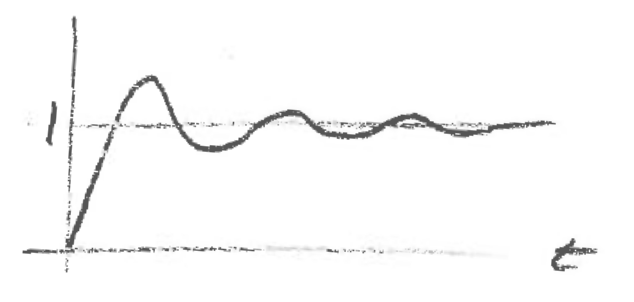
\includegraphics[width=2.5in]{../figures/step_response_2nd_order_with_steady_state_error}
\end{figure}

For a 2\textsuperscript{nd}-order system subjected to a step response, we want to find $x_{ss}$ and $e_{ss}$. Using the transfer function method to solve for the response, we know the system response is
\begin{equation}
x(t) = 1 - \frac{1}{\sqrt{1-\zeta^2}} e^{-\zeta \omega_n t} \sin (\omega_d t + \phi)
\end{equation}
where 
\begin{equation}
\omega_d = \omega_n \sqrt{1-\zeta^2}
\end{equation}
and 
\begin{equation}
\phi = \tan^{-1} \frac{\sqrt{1-\zeta^2}}{\zeta} = \sin^{-1} \sqrt{1-\zeta^2}
\end{equation}
next, the steady-state displacement can be solved for as
\begin{align}
x_{ss} &= \lim\limits_{t \rightarrow \infty} x(t)\\
&= 1 - \frac{\sqrt{1-\zeta^2}}{\zeta}  \lim\limits_{t \rightarrow \infty}  e^{-\zeta \omega_n t} \sin (\omega_d t + \phi) \nonumber \\
&=  1 \nonumber
\end{align}
as $e^{-\zeta \omega_n t} $ goes to 0. Next, the error as a function of time is 
\begin{align}
e(t) &= f(t) - x(t) \\
&= \frac{1}{\sqrt{1-\zeta^2}} e^{-\zeta \omega_n t} \sin (\omega_d t + \phi) \nonumber
\end{align}
while the steady-state error is
\begin{align}
e_{ss} &= \lim\limits_{t \rightarrow \infty}e(t) \\
&=  \frac{\sqrt{1-\zeta^2}}{\zeta}  \lim\limits_{t \rightarrow \infty}  e^{-\zeta \omega_n t} \sin (\omega_d t + \phi) \nonumber \\
&= 0 \nonumber
\end{align}
as $e^{-\zeta \omega_n t} $ goes to 0.


These same solutions can be found in the s-domain where the step function is $F(s)=\frac{1}{s}$. Consider the s-domain expression solved for $X(s)$, 
\begin{equation}
X(s) = \frac{\omega_n^2}{s^2 + 2 \zeta \omega_n s + \omega_n^2} \cdot \frac{1}{s} 
\end{equation}
the steady-state displacement is shown to be
\begin{align}
x_{ss} &= \lim\limits_{s \rightarrow 0} s \frac{\omega_n^2}{s^2 + 2 \zeta \omega_n s + \omega_n^2} \cdot \frac{1}{s} \\
&= \frac{\omega_n^2}{\omega_n^2}   \nonumber \\
&= 1    \nonumber 
\end{align}
Next, we can build the s-domain representation of the error as
\begin{equation}
E(s) = \frac{s^2 + 2 \zeta \omega_n s}{s^2 + 2 \zeta \omega_n s + \omega_n^2} \cdot \frac{1}{s}
\end{equation}
solving for the steady-state error results in
\begin{align}
e_{ss} &= \lim\limits_{s \rightarrow 0} s  \frac{s^2 + 2 \zeta \omega_n s}{s^2 + 2 \zeta \omega_n s + \omega_n^2} \cdot \frac{1}{s} \\
&= \frac{0}{\omega_n}   \nonumber \\
&= 0   \nonumber 
\end{align}

\subsubsection{Impulse response 2\textsuperscript{nd}-order system performance indicators}

\begin{figure}[H]
	\centering
	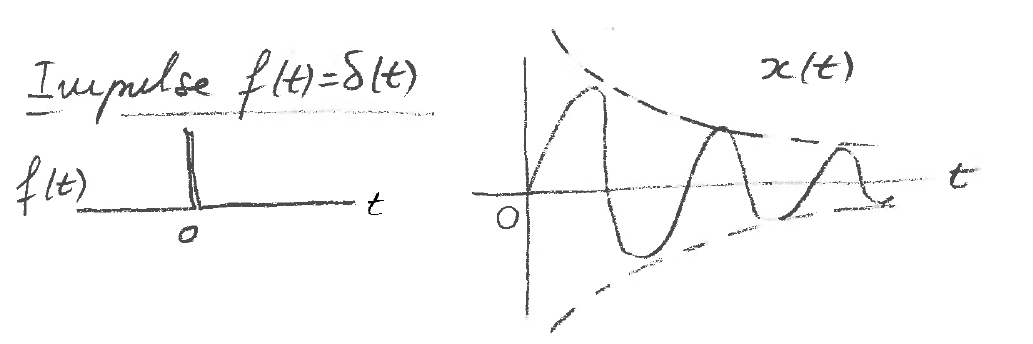
\includegraphics[width=6.5in]{../figures/impulse_response_2nd_order_with_steady_state_error}
\end{figure}



For a 2\textsuperscript{nd}-order system subjected to a impulse response, we want to find $x_{ss}$ and $e_{ss}$. The impulse function is defined as
\begin{equation}
f(t) = \delta(t)
\end{equation}
therefore, the response is
\begin{equation}
x(t) = \frac{\omega_n}{\sqrt{1-\zeta^2}} e ^{-\zeta \omega_n t} \sin(\omega_d t)
\end{equation}
where the steady-state response is
\begin{align}
x_{ss} &= \lim\limits_{t \rightarrow \infty} x(t)\\
&= \frac{\omega_n}{\sqrt{1-\zeta^2}}  \lim\limits_{t \rightarrow \infty}  e^{-\zeta \omega_n t} \sin (\omega_d t + \phi) \nonumber \\
&=  0 \nonumber
\end{align}
as $e^{-\zeta \omega_n t} $ goes to 0. Next, the error as a function of time is 
\begin{align}
e(t) &= f(t) - x(t) \\
&= \delta (t) - \frac{\omega_n}{\sqrt{1-\zeta^2}} e^{-\zeta \omega_n t} \sin (\omega_d t + \phi) \nonumber
\end{align}
Lastly, the steady-state error is
\begin{align}
e_{ss} &= \lim\limits_{t \rightarrow \infty} e(t) \\
&= \lim\limits_{t \rightarrow \infty} \delta (t) - \frac{\omega_n}{\sqrt{1-\zeta^2}} e^{-\zeta \omega_n t} \sin (\omega_d t + \phi) \nonumber \\
&= 0 \nonumber
\end{align}
as $\delta(t)$ and $e^{-\zeta \omega_n t}$ both go to 0. 

These same solutions can be found in the s-domain where the impulse function is $F(s)=1$. Consider the s-domain expression solved for $X(s)$, 
\begin{equation}
X(s) = \frac{\omega_n^2}{s^2 + 2 \zeta \omega_n s + \omega_n^2} 
\end{equation}
the steady-state error is shown to be
\begin{align}
x_{ss} &= \lim\limits_{s \rightarrow 0} s \frac{\omega_n^2}{s^2 + 2 \zeta \omega_n s + \omega_n^2}  \\
&= 0    \nonumber 
\end{align}
The s-domain error is expressed as
\begin{equation}
E(s) = \frac{s^2 + 2 \zeta \omega_n s}{s^2 + 2 \zeta \omega_n s + \omega_n^2}
\end{equation}
which leads to the steady-state error value
\begin{align}
e_{ss} &= \lim\limits_{s \rightarrow 0}  s \frac{s^2 + 2 \zeta \omega_n s}{s^2 + 2 \zeta \omega_n s + \omega_n^2} \\
&= 0   \nonumber 
\end{align}







\subsubsection{Ramp response 2\textsuperscript{nd}-order system performance indicators}

\begin{figure}[H]
	\centering
	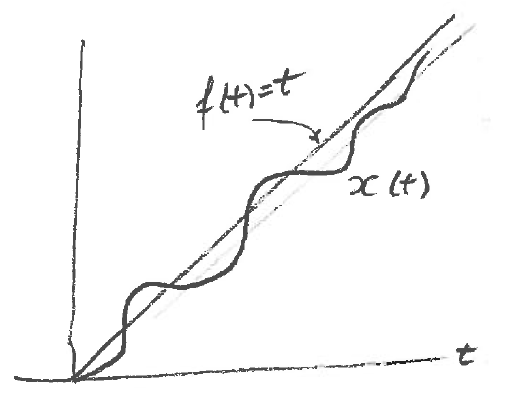
\includegraphics[width=2.5in]{../figures/ramp_response_2nd_order_with_steady_state_error}
\end{figure}

For a 2\textsuperscript{nd}-order system subjected to a ramp response, we want to find $x_{ss}$ and $e_{ss}$. The impulse function is defined as
\begin{equation}
f(t) = t
\end{equation}
therefore, the response can be found through the transfer function approach as
\begin{equation}
x(t) = t - \frac{2 \zeta}{\omega_n} \bigg[ 1 + \frac{1}{\sin \phi_1} e^{-\zeta \omega_n t} \sin (\omega_dt + \phi_1) \bigg]
\end{equation}
where
\begin{equation}
\phi_1 = \tan^{-1} \frac{2 \zeta \sqrt{1-\zeta^2}}{1-2 \zeta ^2}
\end{equation}
which leads to the response
\begin{align}
x_{ss} &= \lim\limits_{t \rightarrow \infty} x(t)  \\
&= t - \frac{2 \zeta}{\omega_n} \nonumber \\
&= \infty \nonumber
\end{align}
which means that there is no steady-state value. Next, the error as a function of time is 
\begin{align}
e(t) &= f(t) - x(t) \\
&= t - \Bigg[ t - \frac{2 \zeta}{\omega_n} \bigg[ 1 + \frac{1}{\sin \phi_1} e^{-\zeta \omega_n t} \sin (\omega_dt + \phi_1) \bigg] \Bigg] \nonumber \\
&= \frac{2  \zeta}{\omega_n} \bigg[ 1 + \frac{1}{\sin \phi_1} e^{-\zeta \omega_n t} \sin (\omega_dt + \phi_1) \bigg]  \nonumber 
\end{align}
Lastly, the steady-state error is
\begin{align}
e_{ss} &= \lim\limits_{t \rightarrow \infty}e(t)  \\
&= \frac{2 \zeta}{\omega_n}   \lim\limits_{t \rightarrow \infty} \bigg[ 1 + \frac{1}{\sin \phi_1} e^{-\zeta \omega_n t} \sin (\omega_dt + \phi_1) \bigg]  \nonumber \\
&= \frac{2  \zeta}{\omega_n} \nonumber
\end{align}
as the term in the brackets goes to 1.

\begin{figure}[H]
	\centering
	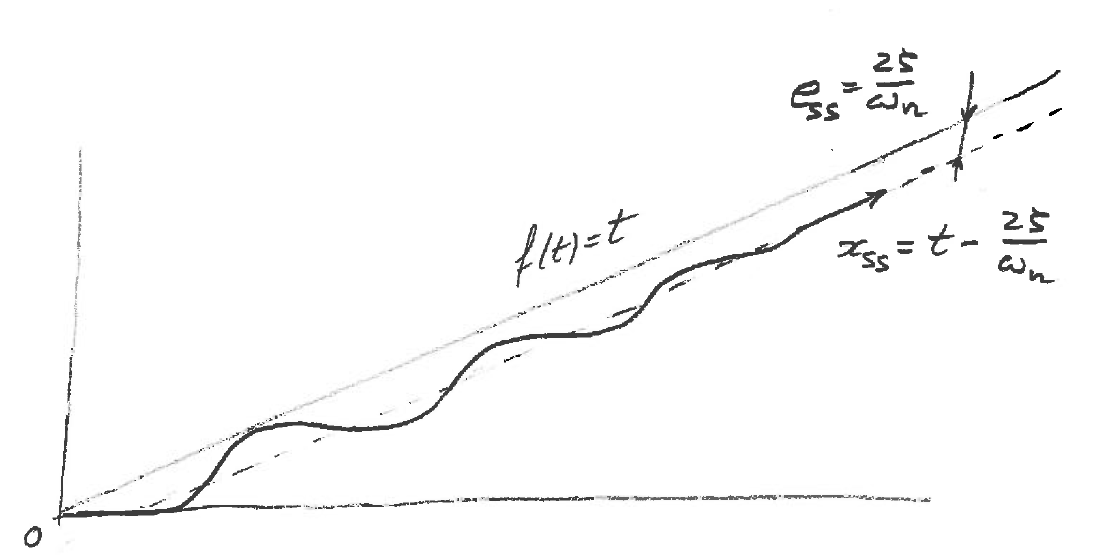
\includegraphics[width=5.5in]{../figures/ramp_response_2nd_order_with_steady_state_error_annotated}
\end{figure}

These same solutions can be found in the s-domain where the ramp function is $F(s)=\frac{1}{s^2}$. Consider the s-domain expression solved for $X(s)$, 
\begin{equation}
X(s) = \frac{\omega_n^2}{s^2 + 2 \zeta \omega_n s + \omega_n^2}  \cdot \frac{1}{s^2} 
\end{equation}
the steady-state error is shown to be
\begin{align}
x_{ss} &= \lim\limits_{s \rightarrow 0} s \frac{\omega_n^2}{s^2 + 2 \zeta \omega_n s + \omega_n^2} \cdot \frac{1}{s^2}  \\
&= \lim\limits_{s \rightarrow 0} \frac{\omega_n^2}{s^2 + 2 \zeta \omega_n s + \omega_n^2} \cdot \frac{1}{s}  \nonumber \\
&= \lim\limits_{s \rightarrow 0}\frac{1}{s}  \nonumber \\
&= \infty  \nonumber
\end{align}
therefore, there is no steady-state value. The s-domain error is expressed as
\begin{equation}
E(s) = \frac{s^2 + 2 \zeta \omega_n s}{s^2 + 2 \zeta \omega_n s + \omega_n^2} \cdot \frac{1}{s^2}
\end{equation}
which leads to the steady-state error value
\begin{align}
e_{ss} &= \lim\limits_{s \rightarrow 0}  s \frac{s^2 + 2 \zeta \omega_n s}{s^2 + 2 \zeta \omega_n s + \omega_n^2} \cdot \frac{1}{s^2} \\
&= \lim\limits_{s \rightarrow 0}   \frac{s^2( s + 2 \zeta \omega_n)}{s^2 + 2 \zeta \omega_n s + \omega_n^2} \cdot \frac{1}{s^2} \nonumber  \\ 
&= \frac{2 \zeta \omega_n}{\omega_n^2}   \nonumber \\
&= \frac{2 \zeta }{\omega_n}   \nonumber
\end{align}

\subsection{2\textsuperscript{nd}-order System Specific Performance Indicators}

\begin{figure}[H]
	\centering
	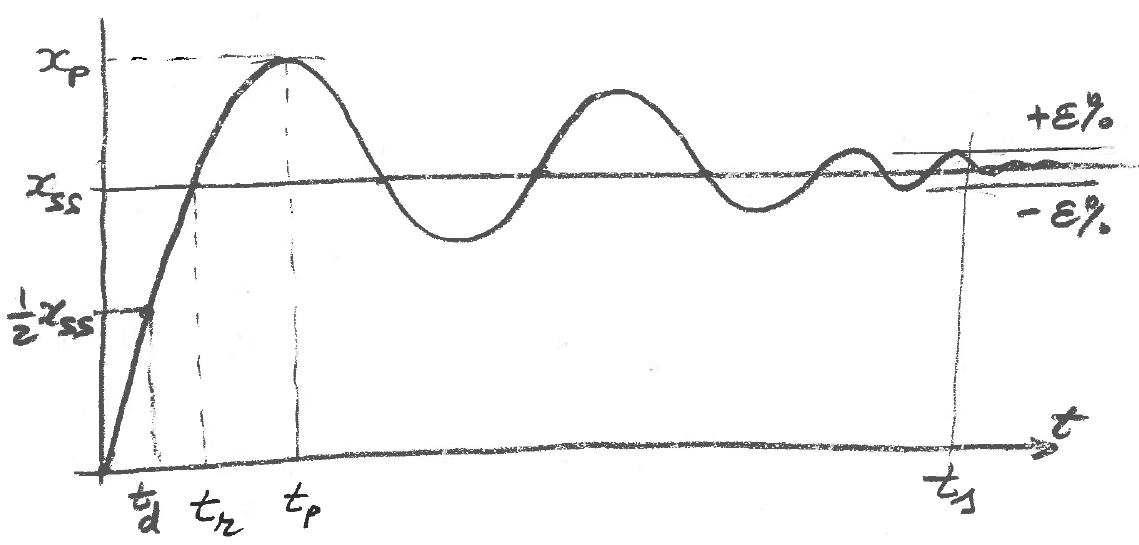
\includegraphics[width=5.5in]{../figures/2nd_order_system_specific_performance_indicators}
\end{figure}

Specific performance indicators exist. They depend on system order and excitation type. Examples are: 
\begin{itemize}
	\item rise time $ \rightarrow t_r$
	\item peak time  $ \rightarrow t_p$
	\item peak value  $ \rightarrow x_p$
	\item settling time $ \rightarrow t_s$
	\item delay time  $ \rightarrow t_d$
	\item max percentage overshoot $ \rightarrow M_p$
\end{itemize}
Many of these are the same as a 1\textsuperscript{st}-order system or taken directly from the system response. The max percentage overshoot ($M_p$) is defined as 
\begin{equation}
M_p = \bigg( \frac{x_p}{x_{ss}}-1 \bigg) \cdot 100
\end{equation}

\subsubsection{Procedure for a Step Response}

Given the 2\textsuperscript{nd}-order system, with the transfer function
\begin{equation}
G(s) = \frac{\omega_n^2}{s^2 + 2 \zeta \omega_n s + \omega_n^2}
\end{equation}
where $\omega_n$ is the natural frequency and $\zeta$ is the critical damping ratio. Considering that the system is subjected to a step response, we know the system response is
\begin{equation}
x(t) = 1 - \frac{1}{\sqrt{1-\zeta^2}} e^{-\zeta \omega_n t} \sin (\omega_d t + \phi)
\label{eq:x_of_t_in_2nd_order_performance}
\end{equation}
where we can calculate:
\begin{equation}
\omega_d = \omega_n \sqrt{1-\zeta^2}
\end{equation}
and
\begin{equation}
\phi = \tan^{-1} \frac{\sqrt{1-\zeta^2}}{\zeta} = \sin^{-1} \sqrt{1-\zeta^2}
\label{eq:tan_in_performance_indicators}
\end{equation}
Next, compute the values for the performance indicators. 

First the rise time is calculated by the fact that $x(0) = 0$ and $x(t_r)=1$. Form equation~\ref{eq:x_of_t_in_2nd_order_performance}, the mean height of the system is shown to be when $ \sin (\omega_d t + \phi) = 0$, therefore, as $\sin(\pi)=0$, we can show that $\omega_d t + \phi = \pi$, rearranging this yields 
\begin{equation}
t_r = \frac{\pi - \phi}{\omega_d}
\end{equation}

To find the peak time ($t_p$), we need to find the peak, which is defined as $\frac{dx}{dt}\big|_{t=t_p} = 0$, or drawn as
\begin{figure}[H]
	\centering
	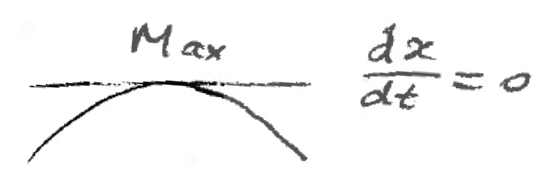
\includegraphics[width=2.5in]{../figures/t_p_max.png}
\end{figure}
where we consider only the decaying part of the signal caused by the step function, or $x=e^{-\zeta \omega_n t} \sin (\omega_d t + \phi)$. Therefore
\begin{align}
0 &= \frac{dx}{dt}  \\
 &= \frac{d}{dt} \bigg[  e^{-\zeta \omega_n t} \sin (\omega_d t + \phi)   \bigg]  \nonumber \\
 &= - \zeta \omega_n e^{-\zeta \omega_n t} \sin (\omega_d t + \phi) + \omega_d e^{-\zeta \omega_n t} \cos (\omega_d t + \phi) \nonumber \\
\zeta \omega_n \sin (\omega_d t + \phi) &= \omega_d \cos (\omega_d t + \phi) \nonumber \\
\frac{\sin (\omega_d t + \phi)}{\cos (\omega_d t + \phi)} & = \frac{\omega_d}{\zeta \omega_n}  \nonumber
\end{align}
By converting the left has side of this equation to $\tan (\omega_d t_p + \phi)$ yields
\begin{align}
\label{eq:tan_of_phi}
\tan (\omega_d t_p + \phi) &= \frac{\omega_d}{\zeta \omega_n} \\
&= \frac{\sqrt{1-\zeta^2} }{\zeta} \nonumber \\
&= \tan(\phi) \nonumber
\end{align}
when considering the definition of tan provided by equation~\ref{eq:tan_in_performance_indicators}. We must find $t_p$ such that $\tan(\omega_d t_p + \phi) = \tan(\phi)$. Given that the function $\tan(\alpha)$ repeats itself after $\pi, \; 2\pi, \; 3\pi, \; \cdots$ as shown in figure~\ref{fig:tan_of_alpha}, we know $\tan(\alpha) = \tan(\alpha + \pi) = \tan(\alpha + 2\pi), \cdots $.  
\begin{figure}[H]
	\centering
	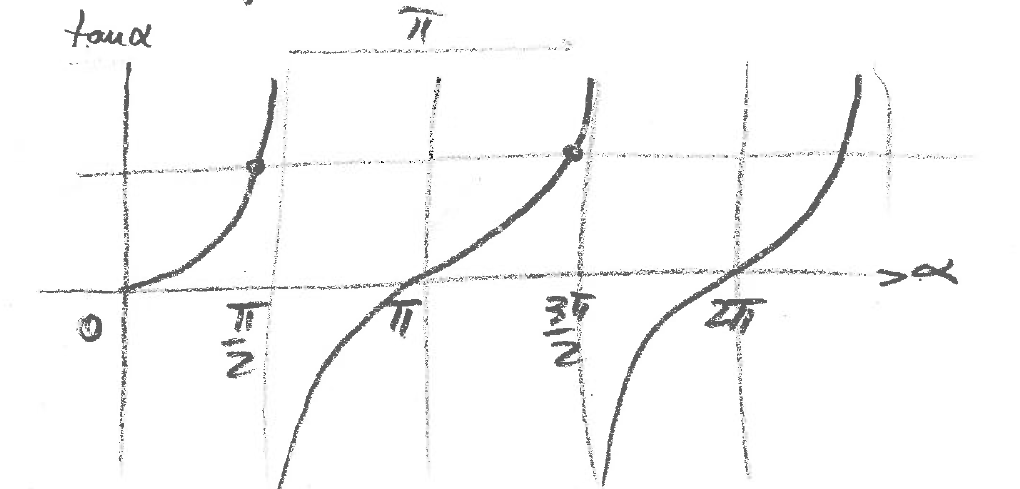
\includegraphics[width=4.5in]{../figures/tan_of_alpha.png}
	\caption{Plotting the $ \tan(\alpha)$}
	\label{fig:tan_of_alpha}
\end{figure}
\noindent Hence, picking back up from equation~\ref{eq:tan_of_phi} lead to
\begin{align}
\omega_d t_p + \phi &= \phi + \pi\\
\omega_d t_p &= \pi \nonumber 
\end{align}
which results in
\begin{equation}
t_p = \frac{\pi}{\omega_d}
\end{equation}



The peak value ($x_p$) can be found as
\begin{align}
x_p &= x(t_p) \\
&= 1 - \frac{1}{ \sqrt{1-\zeta^2}} e^{-\zeta \omega_n \frac{\pi}{\omega_d}} \sin\big(\omega_d (\sfrac{\pi}{\omega_d}) + \phi \big)\nonumber \\
&= 1 + \frac{1}{ \sqrt{1-\zeta^2}} e^{-\zeta \omega_n \frac{\pi}{\omega_d}} \sin(\phi)\nonumber \\
&= 1 + \frac{1}{ \sqrt{1-\zeta^2}} \bigg( e^{- \frac{\zeta}{\sqrt{1-\zeta^2}} \pi} \bigg) \sqrt{1-\zeta^2} \nonumber \\
&= 1 + e^{- \frac{\zeta}{\sqrt{1-\zeta^2}} \pi} \nonumber
\end{align}
when considering that $\sin(\phi + \pi) = -\sin(\phi)$ and $\sin(\phi) = \sqrt{(1-\zeta^2)}$.


The max overshoot ($M_p$) can be found as
\begin{align}
M_p &= \frac{x_p - x_{ss}}{x_{ss}} \\
&= \frac{1 + e^{\frac{\zeta}{\sqrt{1-\zeta^2}}\pi} -1 }{1} \nonumber \\
&= e^{- \frac{\zeta}{\sqrt{1-\zeta^2}} \pi } \nonumber 
\end{align}
for a few select damping ratios, the overshoot percentages are shown in Table~\ref{table:mp_and_damping_ratio}. However, the typical range of damping is $0.4 < \zeta < 0.8$ and therefore the typical max overshoot is $0.25\% < M_p < 1.5\%$.
\begin{table}[H]
\centering
\caption{Overshoot percentages for select damping ratios.}
\label{table:mp_and_damping_ratio}
\begin{tabular}{@{}lcccccc@{}}
\toprule
$\zeta$ & 0 & 0.2 & 0.4 & 0.6 & 0.8 & 1 \\ \midrule 
$M_p$ & 100.00\% & 52.68\% & 25.40\% & 9.49\% & 1.52\% & 0.00\% \\ \bottomrule
\end{tabular}
\end{table}



The definition of settling time $(t_s)$ is to ``get withing $\pm \epsilon \%$ of $x_{ss}$ and stay so''. 
\begin{figure}[H]
	\centering
	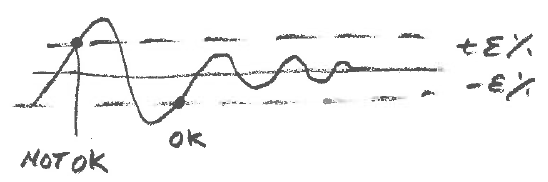
\includegraphics[width=3.5in]{../figures/2nd_order_settling_time_definition.png}
\end{figure}
\noindent The settling time is defined as the time when both 
\begin{equation}
|x_{ss} - x(t_s)| < \Delta
\end{equation}
and
\begin{equation}
|x_{ss} - x(t > t_s)| < \Delta
\end{equation}
are true where $\Delta = \epsilon \cdot x_{ss}$. This is shown in figure~\ref{fig:2nd_order_settling_time}.
\begin{figure}[H]
	\centering
	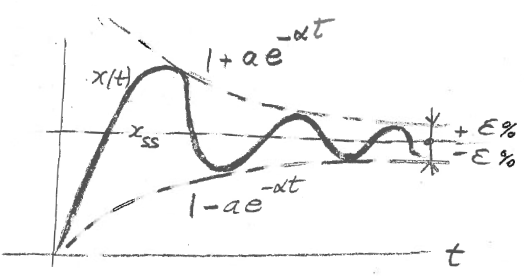
\includegraphics[width=3.5in]{../figures/2nd_order_settling_time.png}
	\caption{Settling time for a 2\textsuperscript{nd}-order system.}
	\label{fig:2nd_order_settling_time}
\end{figure}
\noindent We can find a generalized expression for $t_s$ if we consider the system response for $x_{ss} = 1$ as
\begin{equation}
x(t) = 1 - \bigg[\frac{1}{\sqrt{1-\zeta^2}} \bigg] e^{-[\zeta \omega_n] t} \sin(\omega_d t+ \phi)
\end{equation}
redefining the items in the brackets as $a$ and $\alpha$, respectively, the system response can be simplified to
\begin{equation}
x(t) = 1 - a e^{-\alpha t} \sin(\omega_d t+ \phi)
\end{equation}
Therefore, the envelop of the system response is $1\pm a e^{- \alpha t}$ while the settling condition is $a e^{- \alpha t} = \Delta$. Considering that the final peak aboove the error range will happen when $a \approxeq 1$, we make the approximate calculation
\begin{equation}
a = \frac{1}{\sqrt{1-\zeta^2}}\bigg|_{\zeta << 1} \approxeq 1
\end{equation}
and considering that $t_s$ is when the system decays under the value $\epsilon$, we need to find the $t$ value when
\begin{equation}
e^{- \alpha t} = \epsilon
\end{equation}
therefore, setting $\epsilon =2\%$, we can find
\begin{align}
e^{- \alpha t} &= 0.02 \\
- \alpha t &= \log(0.02) \\
&= -3.9 \nonumber \\
&\approxeq -4 \nonumber
\end{align}
Therefore, knowing that $\alpha = \zeta \omega_n$, we can deduce
\begin{align}
- \alpha t_s &\approxeq -4 \\
- \zeta \omega_n t_s &\approxeq -4 \nonumber \\
t_s &\approxeq \frac{4}{\zeta \omega_n} \nonumber
\end{align}
when $\zeta << 1$ this simplified expression is within $\pm 2\%$.

Importantly, one should always consider the effects of $\zeta$ and $\omega_n$ on performance. 
\begin{itemize}
\item An increase in $\omega_n$ shortens rise time ($t_r$), peak time ($t_p$), and settling time ($t_s$).
\item An increase in $\zeta$ reduces max overshoot ($M_p$) and shortens settling time ($t_s$).
\end{itemize}

As before, the definition of time delay ($t_d$) for a 2\textsuperscript{nd}-order system  is the time it takes to rise to 50\% of $x_{ss}$ the first time. Similarly, the max percentage overshoot ($M_p$) for a 2\textsuperscript{nd}-order system is calculated in the same way as a 1\textsuperscript{st}-order system.







\begin{example}

\textbf{SIMULINK Tutorial on Measuring Performance Indicators}

Build the simple 2\textsuperscript{nd}-order system as shown below
\begin{figure}[H]
	\centering
	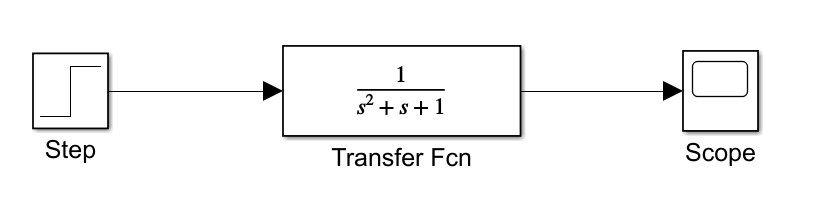
\includegraphics[width=4.5in]{../figures/Simulink_step_model_transfer_2nd_oder}
\end{figure}
Open the scope and press the `Cursor Measurements' button to activate the cursors.

\begin{figure}[H]
	\centering
	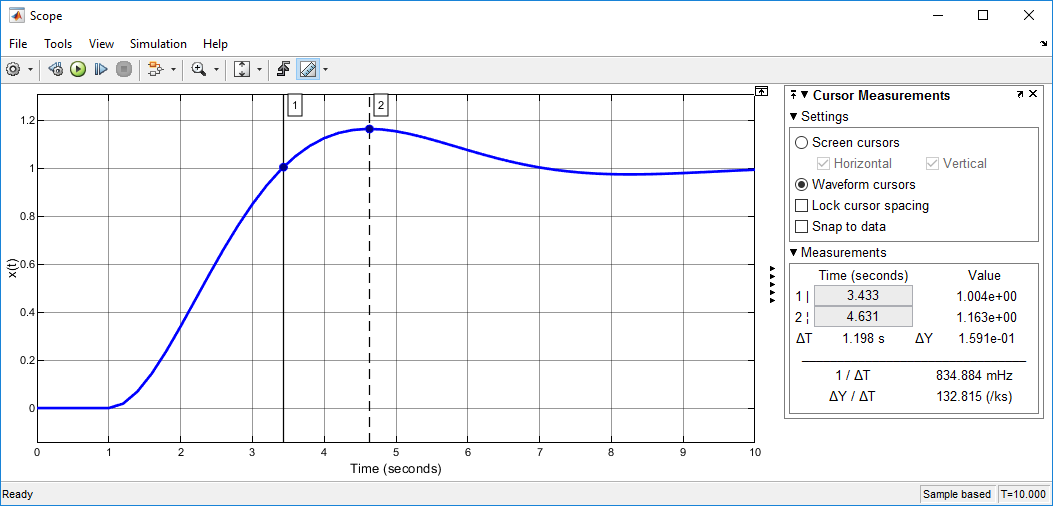
\includegraphics[width=6.0in]{../figures/Simulink_step_model_transfer_cursor_measurements_2nd_oder}
\end{figure}

Use the first cursor to find the first crossing of $x_{ss} = 1$ . Read the time as $t_r = 2.433$ sec as the step function starts at 1 sec. Place the second cursor at peak value. Read the peak time $t_r = 3.631$ sec and peak amplitude
$x_p = 1.163$ . Calculate $M_p = 16.3\%$.

\end{example}


	\pagebreak
	\renewcommand{\thepage}{}
	\renewcommand\refname{References Cited}
	\pagestyle{plain}
	\bibliographystyle{Downey_NSF}
	\bibliography{Chapter_1_Basic_Concepts}


















\end{document}

